\chapter{Modulare Anlage}
\section{Zustandsmodell Services}
\label{A:Zustandsmodell-Services}

 \begin{figure}[htbp]
 \centering
 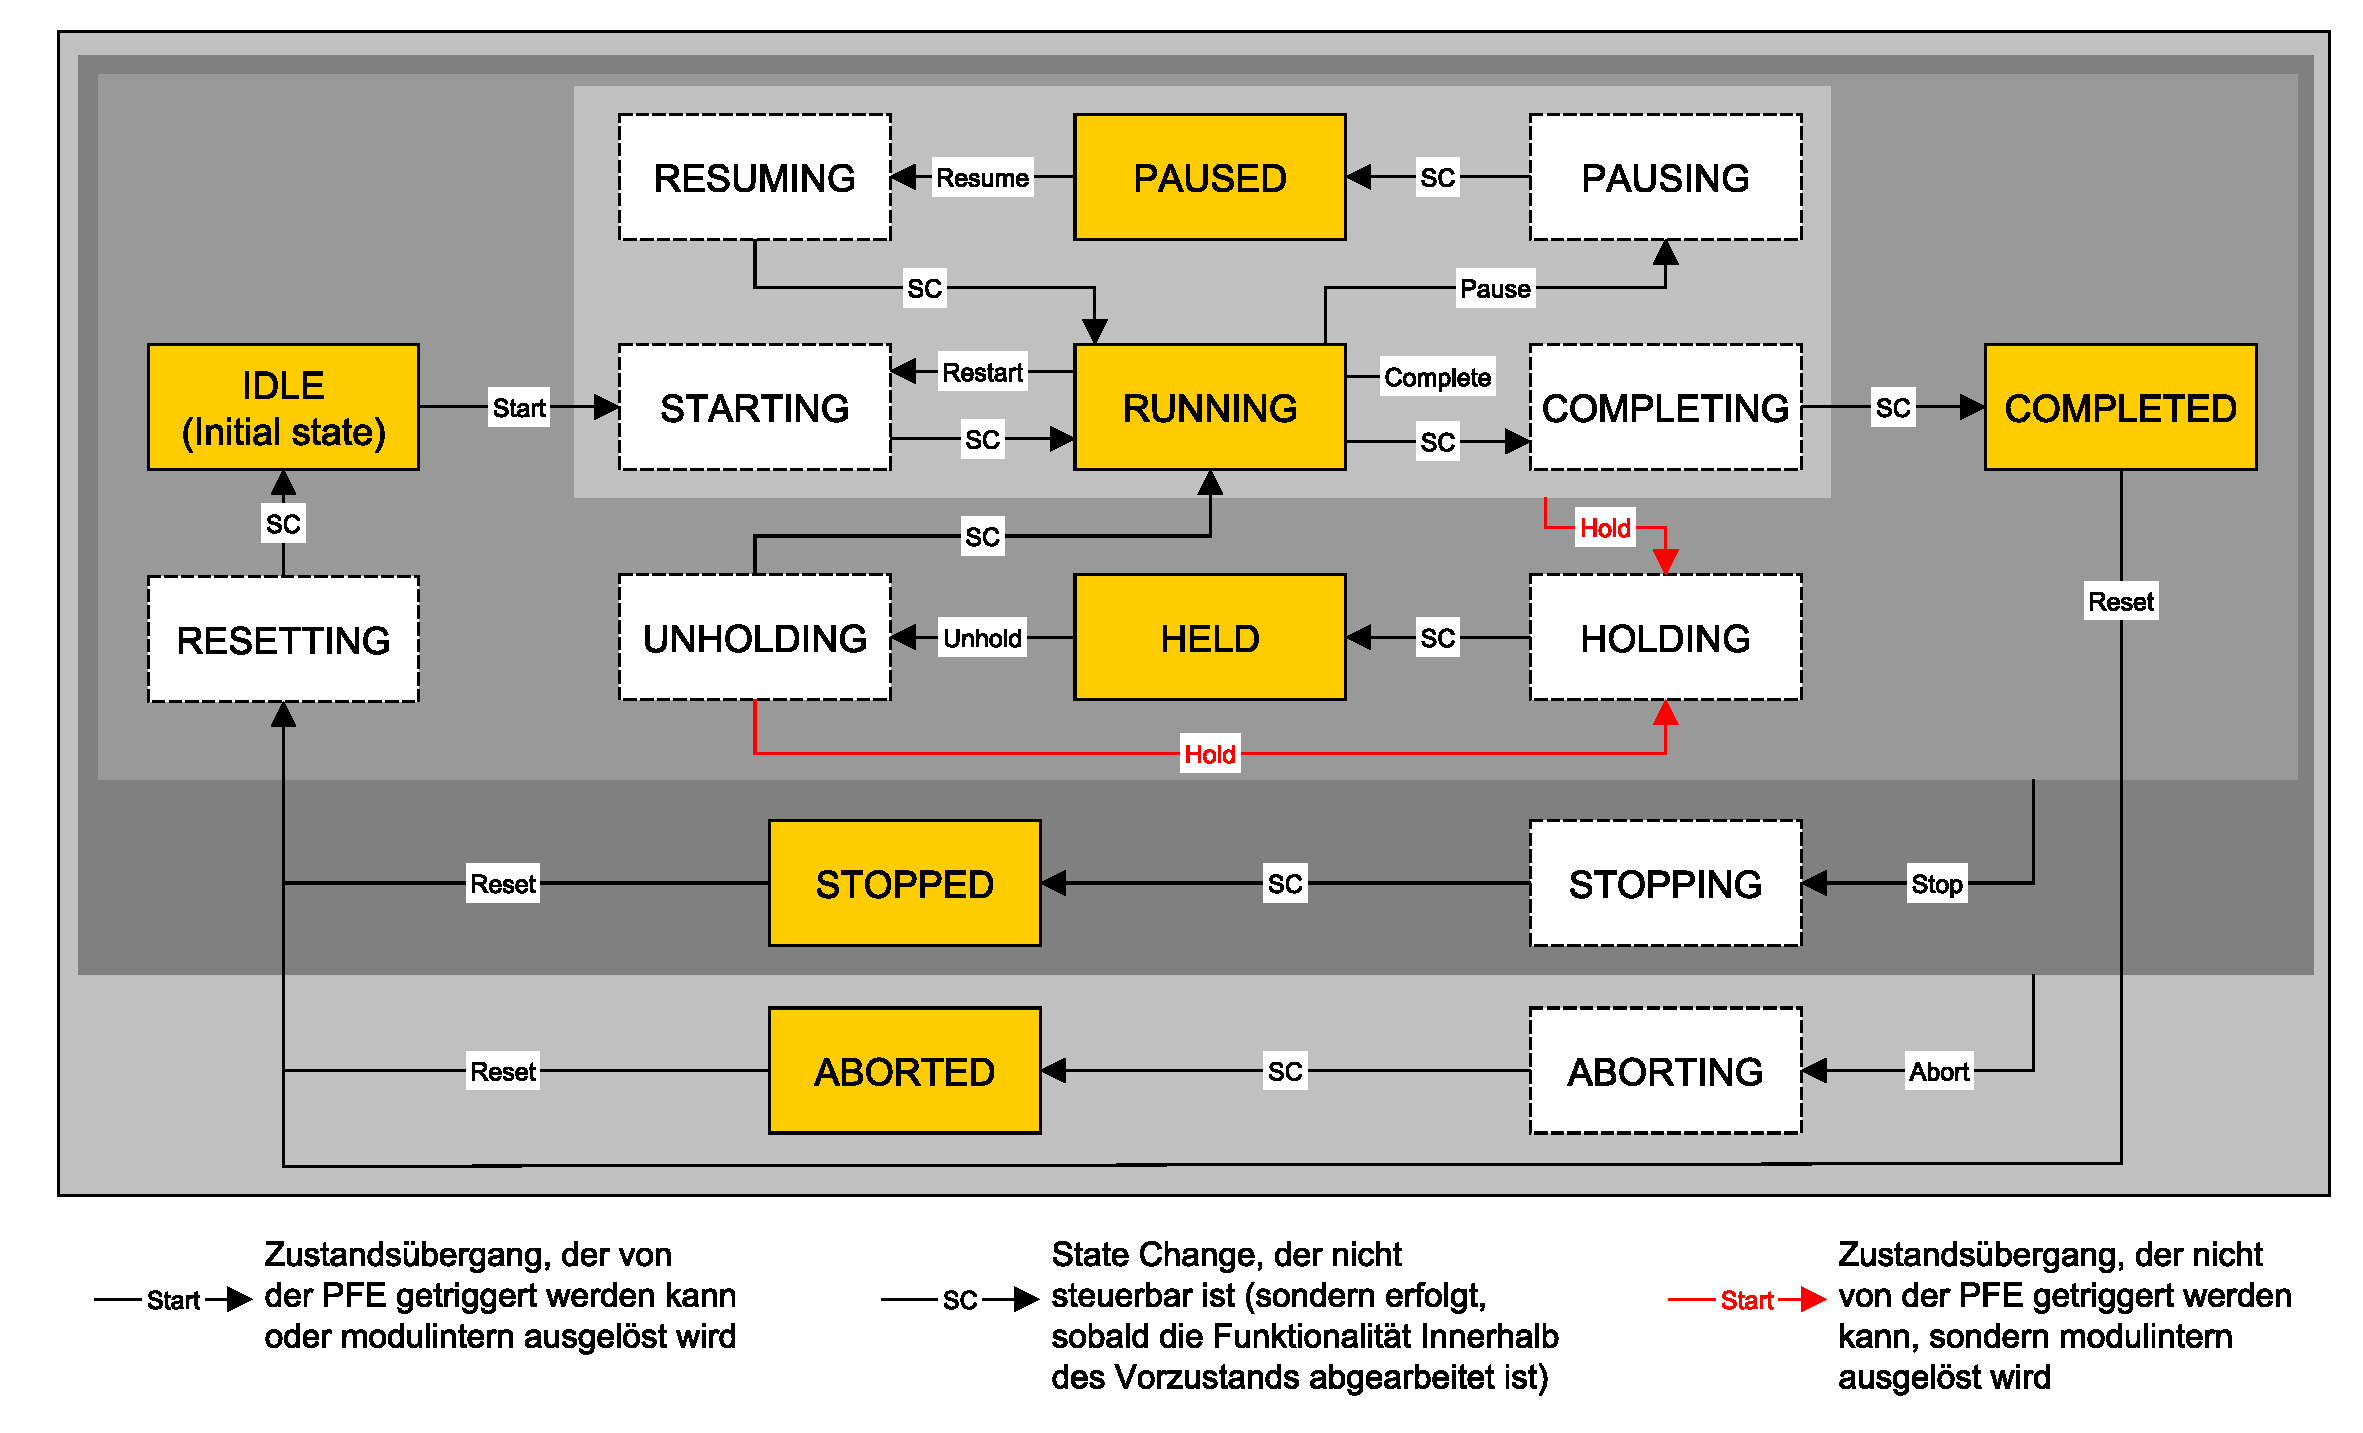
\includegraphics[scale=0.31]{DA_files/Bilder/Anhang/Zustandsdiagramm-Services.pdf}
 \caption[Zustandsmodell Services \textit{nach VDI 2658 Blatt 4}]{Zustandsmodell Services \textit{nach VDI 2658 Blatt 4} \citep[]{VDI2658-Blatt4}}
 \label{pic:Zustandsmodell-Service}
 \end{figure}

\section{Rezept}
\begin{figure}
\centering
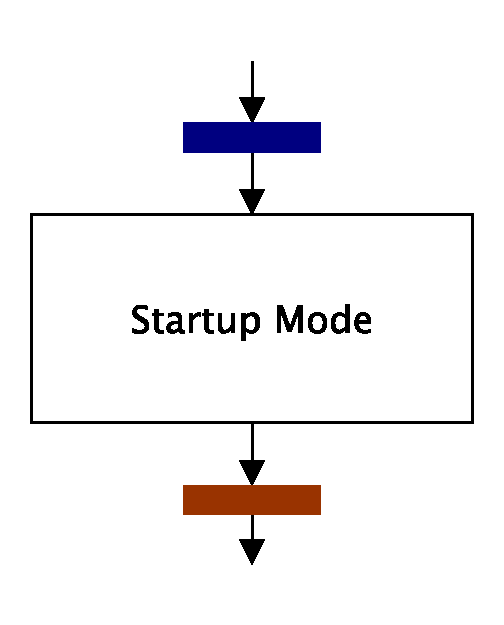
\includegraphics[scale=0.37]{DA_files/Bilder/Anhang/Phases.pdf}
\caption[Rezeptstruktur modulare Anlage - Phases \textit{nach Bloch et.al.}]{Rezeptstruktur - Phases \textit{nach Bloch et.al.} \citep[53]{Bloch2017}}
\end{figure}

\begin{figure}
\centering
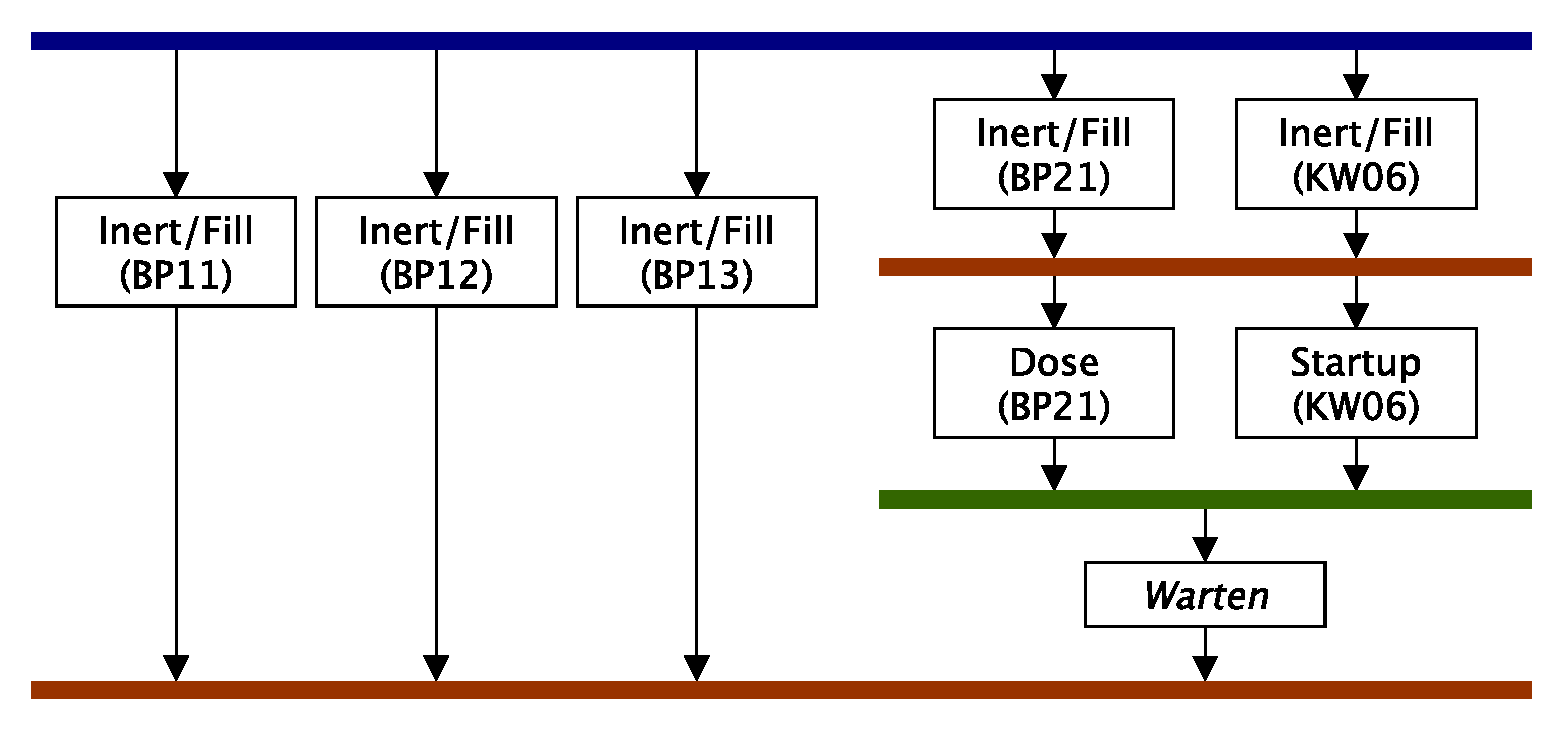
\includegraphics[scale=0.37]{DA_files/Bilder/Anhang/Procedures.pdf}
\caption[Rezeptstruktur modulare Anlage - Procedures \textit{nach Bloch et.al.}]{Rezeptstruktur - Procedures \textit{nach Bloch et.al.} \citep[53]{Bloch2017}}
\end{figure}

\begin{figure}
\centering
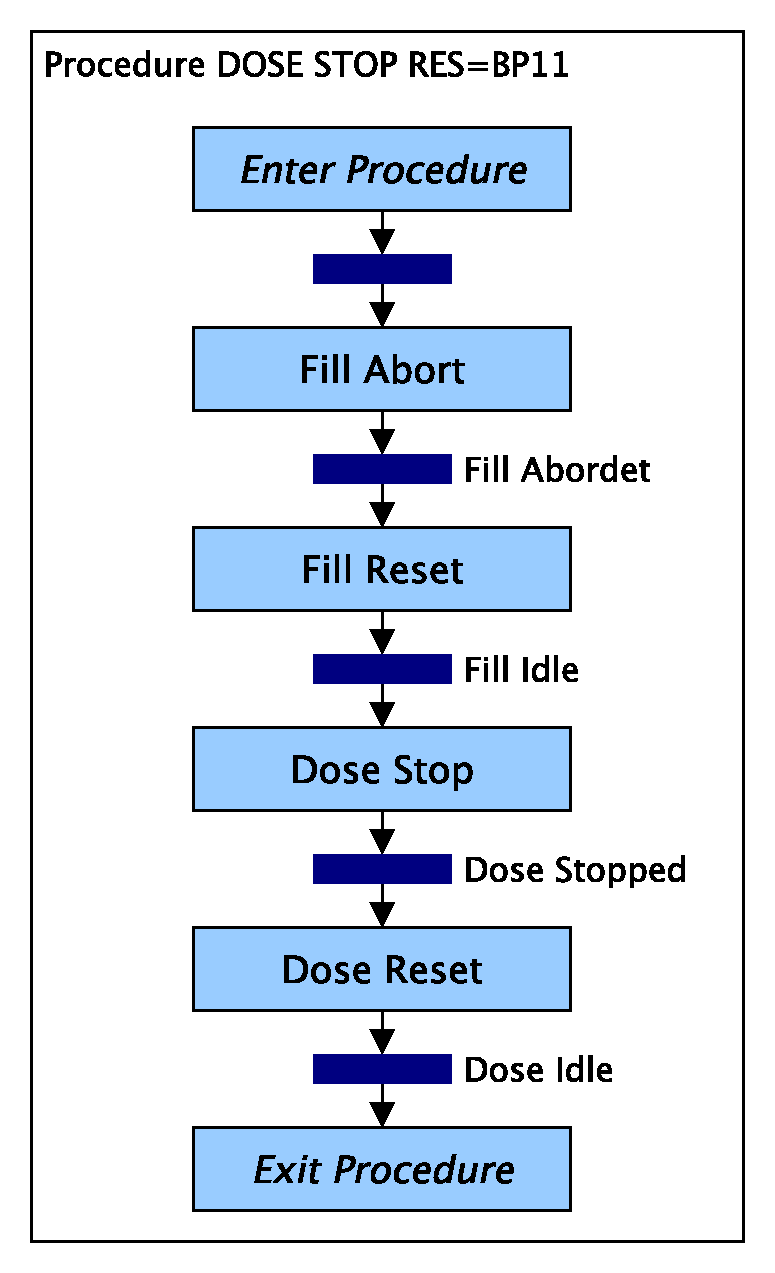
\includegraphics[scale=0.28]{DA_files/Bilder/Anhang/Steps.pdf}
\caption[Rezeptstruktur modulare Anlage - Steps \textit{nach Bloch et.al.}]{Rezeptstruktur - Steps \textit{nach Bloch et.al.} \citep[53]{Bloch2017}}
\end{figure}

\chapter{Prozessführungsebene}
\label{A:PFE}
Für eine besser Übersicht ist die PFE in vier Ebenen eingeteilt. Auf der obersten Ebene ist eine grobe Übersicht über die Anlage gegeben. Die unterste Ebene stellt die meisten Details dar. Tabelle \ref{tab:Ebenen-PFE} beschreibt, welche Informationen auf welcher Ebene dargestellt sind. Mittels der Navigation können die Ebenen gewechselt werden.
\begin{table}[htbp]
\caption{Übersicht über die Ebenen in der Prozessführungsebene}
\centering
\begin{tabular}{p{1,7cm}|p{2,3cm}|p{2,2cm}|p{2,2cm}|p{2,3cm}|}
 & \textbf{Navigation} & \textbf{KPI} & \textbf{Rezept} & \textbf{Services / HMI} \\
\hline
\textbf{Ebene 1} & Shopfloor: Übersicht über alle vorhandenen Anlagen & & Phases für die angewählt Anlage & / \\
\hline
\textbf{Ebene 2} & Subplant: Anzeige aller Module und deren Verbindungen &  & Procedures & Alle Services der Anlage \\
\hline
\textbf{Ebene 3} & Modul & KPIs für das angewählte Modul & Procedures: Markierung des angewählten Moduls & Services des Moduls \\
\hline \textbf{Ebene 4} & Modul & & Procedures: Markierung des Moduls & Anzeige des HMI des Moduls \\
\hline
\end{tabular}
\label{tab:Ebenen-PFE}
\end{table}

\todo{Bilder PFE}

\chapter{Konzept}
\section{Farbschema des Assistenzsystems}
\label{A:Farbschema-Assistenz}
\begin{table}[htb]
\begin{tabular}{l|l|l|l|}
Farbe & \cellcolor{darkgreen}{\color{white}689F38} & \cellcolor{green}{\color{white}689F38} &  \cellcolor{lightgreen}{689F38}\\
\hline
Anwendung & Header & & Buttons\\
\end{tabular}
\end{table}

\section{Anpassung an Problembereich - Aktivitätsdiagramm}
\begin{figure}[hb]
\centering
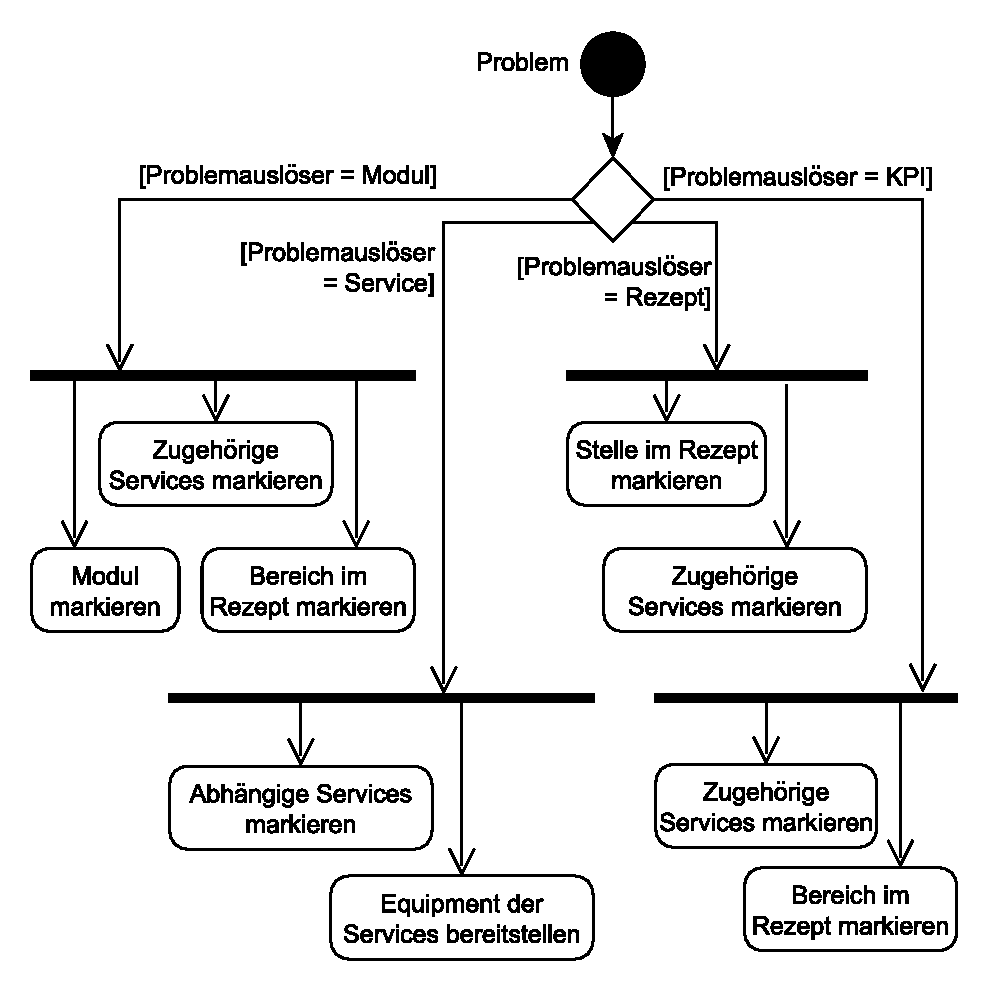
\includegraphics[scale=0.6]{DA_files/UML/Anhang/Aktivitaetsdiagramm-Problem.pdf}
\caption{Aktivitätsdiagramm - Anpassung an Problemauslöser}
\end{figure}

\chapter{Fragebogen}
\label{A:Fragebogen-Validierung}
%\section{Fragebogen User Experience}

\begin{figure}[htbp]
\centering
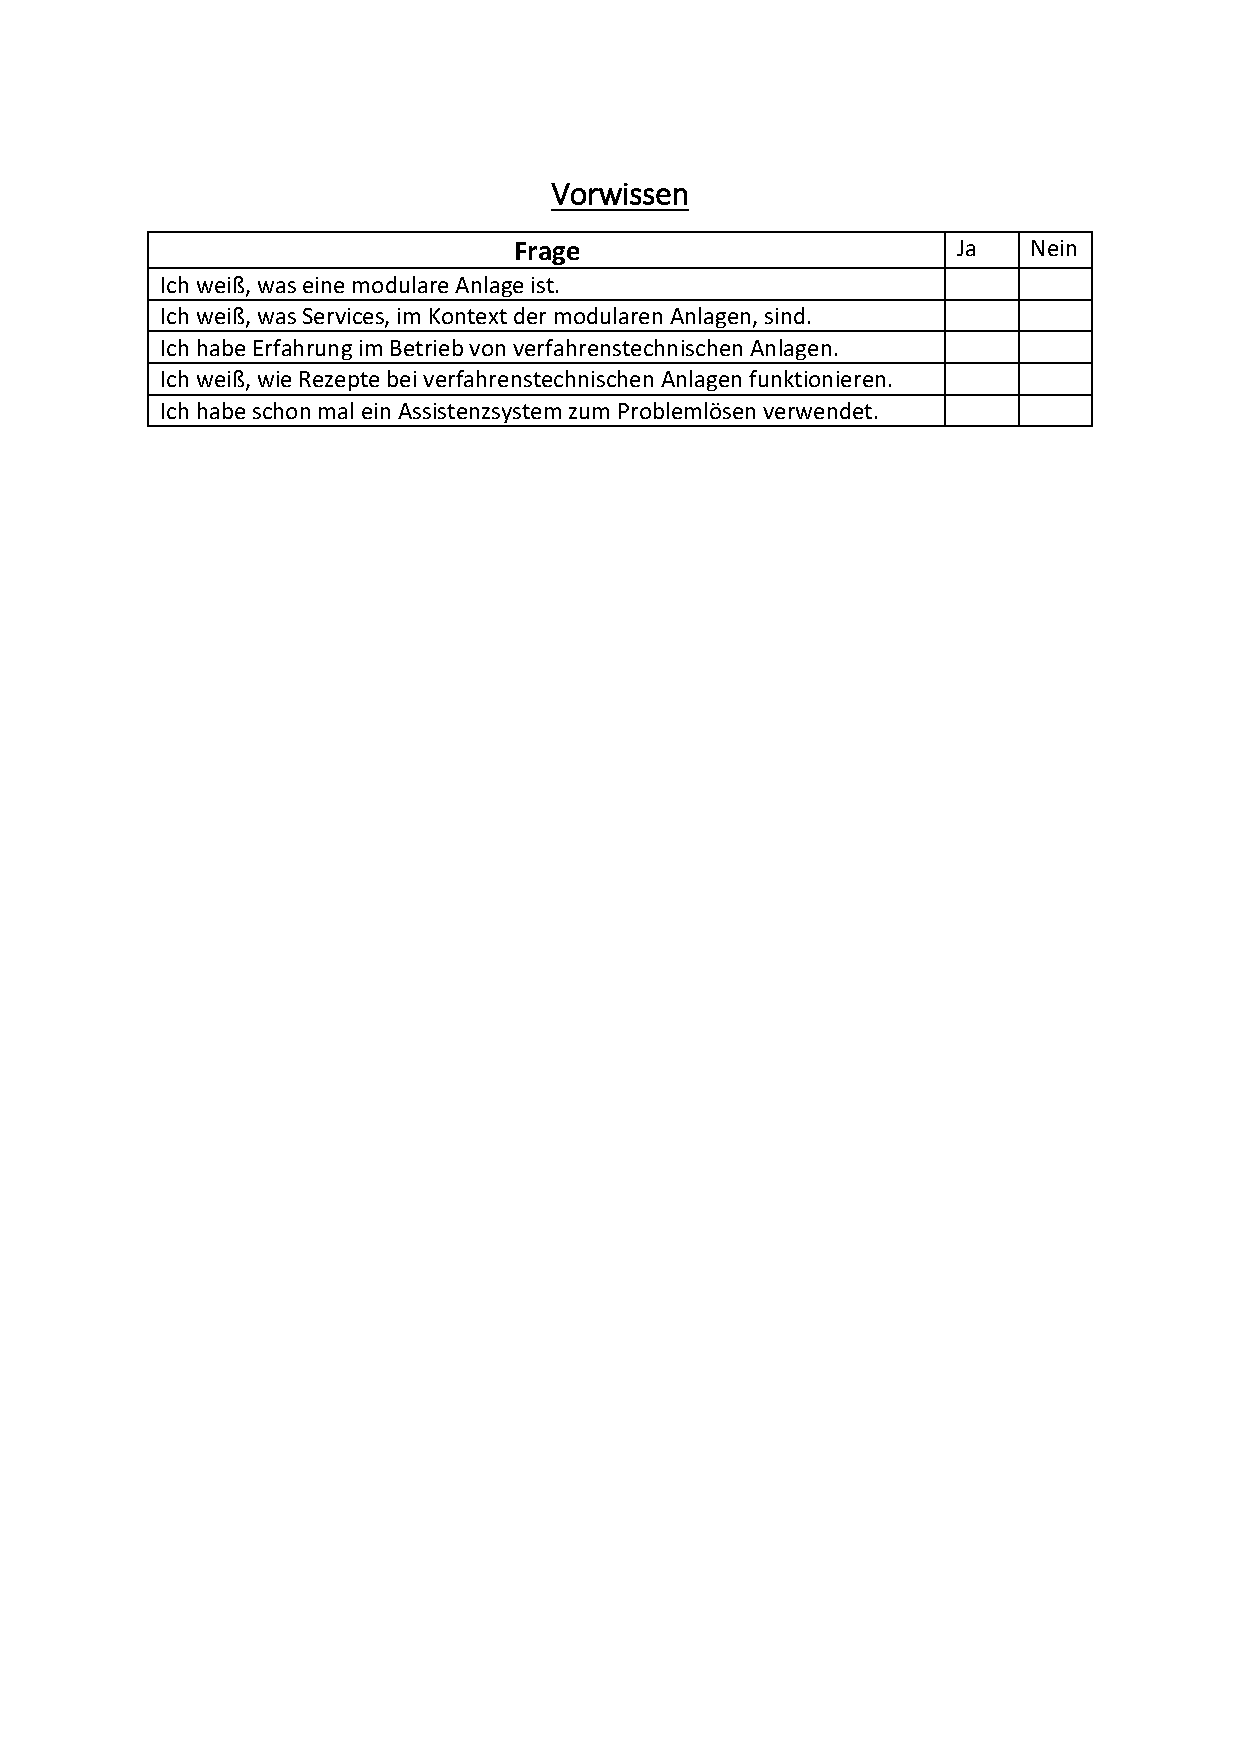
\includegraphics[scale=0.8]{DA_files/Bilder/Anhang/Fragebogen-Vorwissen.pdf}
\caption{Aussagen zum Vorwissen}
\end{figure}

\begin{figure}[htbp]
\centering
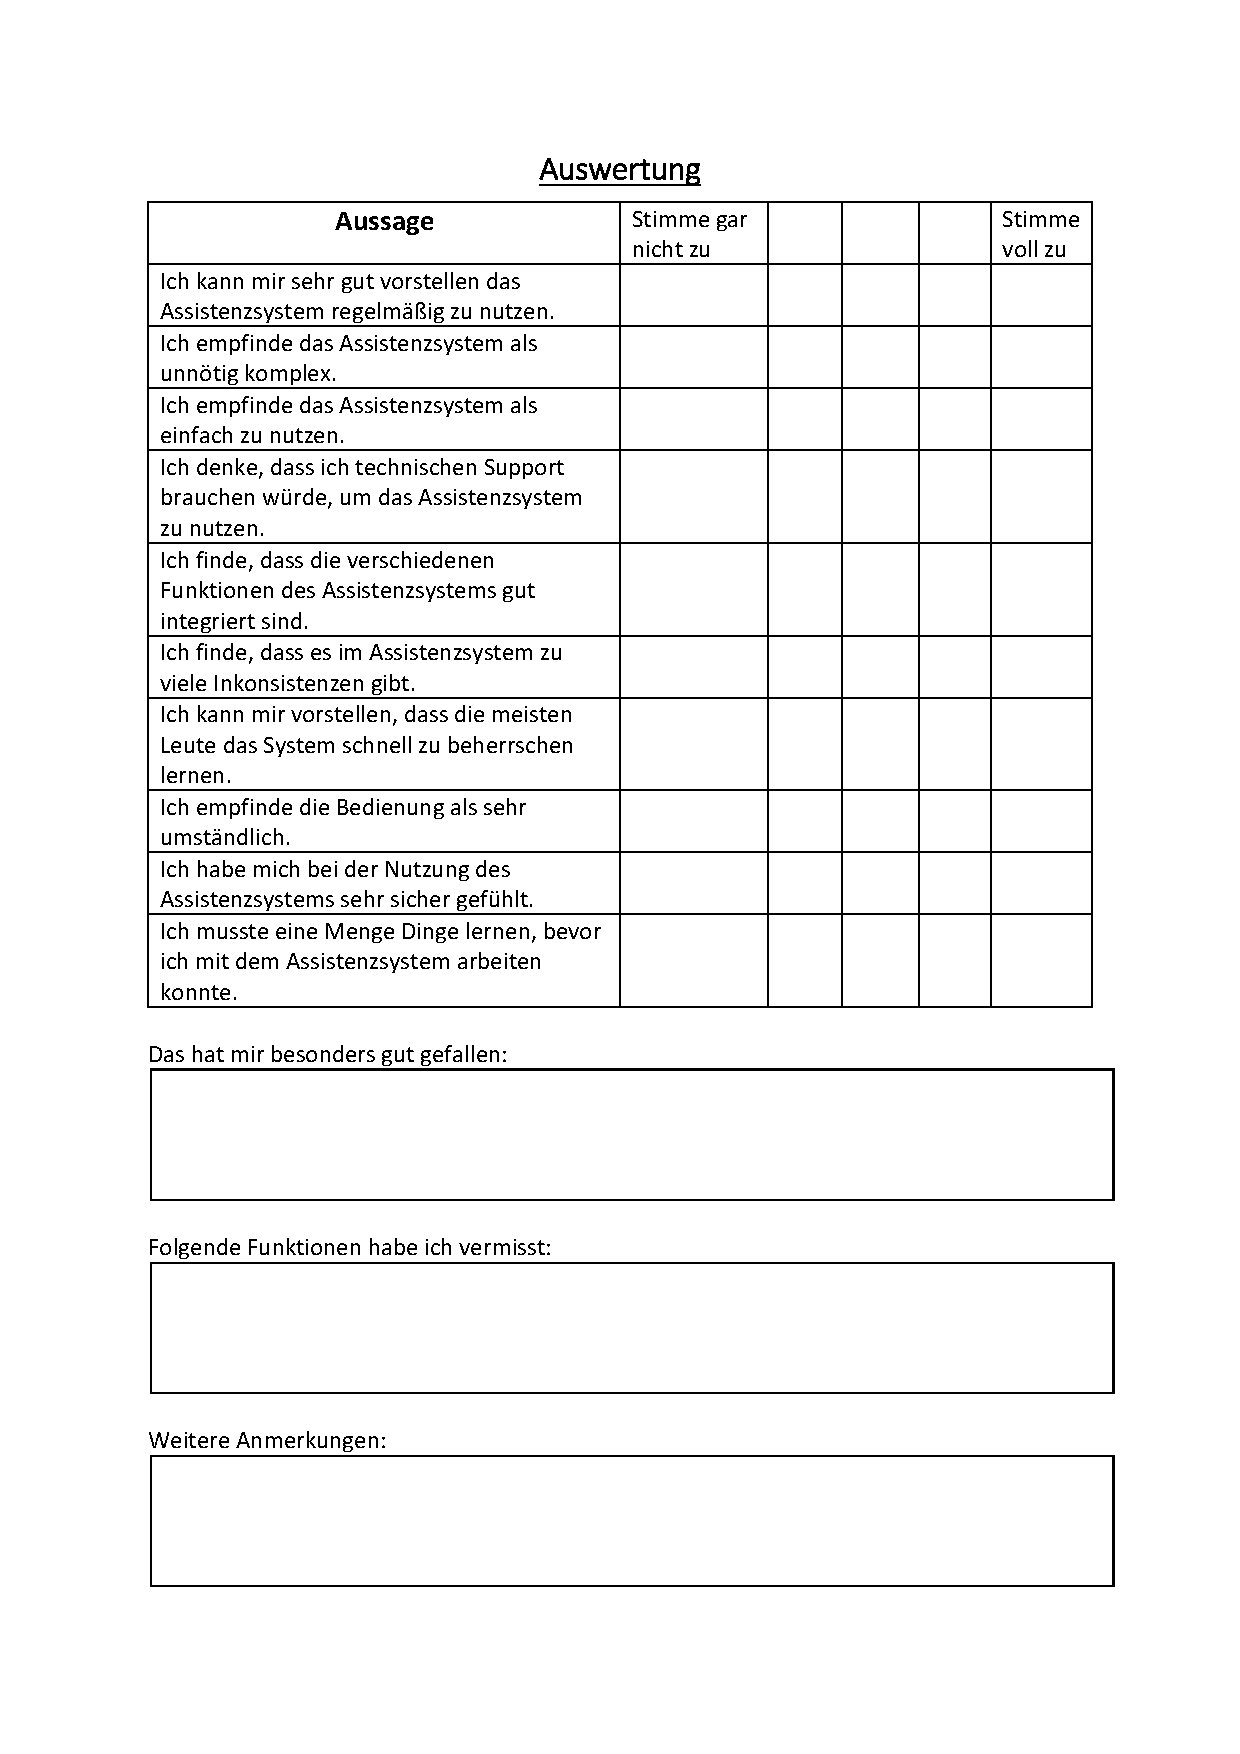
\includegraphics[scale=0.8]{DA_files/Bilder/Anhang/Fragebogen-Auswertung.pdf}
\caption{Auswertung}
\end{figure}

